\documentclass[minimal]{standalone}
\usepackage{tikz}
\begin{document}
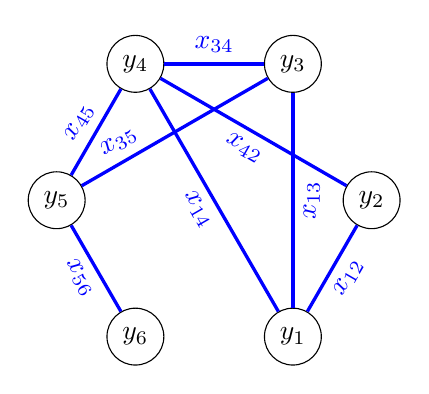
\begin{tikzpicture}
[every edge/.append style={color=blue,very thick},
]
\def \n {6}
\def \radius {2cm}
\def \margin {8} % margin in angles, depends on the radius
\foreach \s in {1,...,\n}
{
{\node[draw, circle] (\s) at ({360/\n * (\s - 2)}:\radius)  {$y_{\s}$};}
} 


\draw  (1) edge node [midway,below,sloped] {$x_{12}$}   (2); 
\draw  (4) edge node [midway,below,sloped]  {$x_{42}$} (2) ;  
\draw  (1) edge node [midway,below,sloped]  {$x_{13}$} (3)   ;  
\draw  (1) edge node [midway,below,sloped]   {$x_{14}$} (4) ;  
\draw  (4) edge node [midway,above,sloped]   {$x_{45}$}   (5);  
\draw  (3) edge node [near end,above,sloped] {$x_{35}$}  (5)  ; 
\draw  (6) edge node [midway,below,sloped]   {$x_{56}$}  (5) ;  
\draw  (3) edge node [midway,above,sloped]  {$x_{34}$}  (4) ; 
\end{tikzpicture}

\end{document}
